\newcommand{\myCoord}[1]{
  \tikz[remember picture]{\coordinate[remember picture] (#1) at (0,0);
    %\fill[red] (#1) circle[radius=1pt];
  }
}


\begin{tikzpicture}[remember picture]
  \tikzstyle{noMargin} = [inner sep=0mm, outer sep=0mm]
  \node[draw,noMargin, remember picture, anchor=north west](methodTech){
    \begin{tabular}{lc}
      technology used for:&\\ 
      \qquad detection& \myCoord{mlInit}\\
      \qquad segmentation&\\
      \qquad post-processing&\myCoord{mlFin}\\
      \multicolumn{2}{l}{$\mathcal{S}$:~Quick-Shift super-pixels}\\
      $\arg \min (U(\cdot))$:\\
      \qquad methodology&\acl{gc}\\
      \qquad design constrains&\tikz{\draw (0,0) -- (15pt,0);}\\
      $D(\cdot)$:\\
      \qquad visual cues& \tikz[noMargin, baseline=(img.north)]{\node[noMargin](img){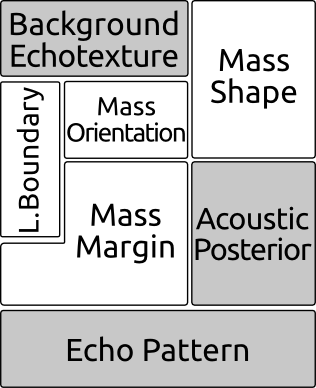
\includegraphics[width=1cm]{vcues}};}\\
      \qquad design constrains&\tikz{\draw (0,0) -- (15pt,0);}\\
      $V(\cdot,\cdot)$:\\
      \qquad visual cues& \tikz{\draw (0,0) -- (15pt,0);}\\
      \qquad design constrains& Homogenity\\
    \end{tabular}
  };
  \node[yshift=2pt,remember picture, overlay, nodeBase, mlStyle, fit= (mlInit) (mlFin)]{};

  \node[draw, right= of methodTech](testingNode){
    \begin{tabular}{l}
      Database size: $16$ \\
      \ac{gt}: multi-label \\
      Task: $\mathcal{L} = \{\text{lesion}, \overline{\text{lesion}}\}$ \\
      Trainning: Leave-one-Patient-Out
    \end{tabular}
    };
    \node[draw, noMargin, below= 0pt of testingNode](resultsNode){
      \begin{tabular}{lc}
        \ac{aov}& .623 \\
        \ac{fpr}& .4 \\
        \ac{fnr}& .008 \\
      \end{tabular}
  };
\node[
      draw=red,
      minimum width=\textwidth,
      fit=(current bounding box.north west) (current bounding box.south east),
    ]at (current bounding box.center){};
\end{tikzpicture}

